\documentclass{article}
\usepackage{listings}
\usepackage{graphicx}
\author{Yuxiang Chen 5110309783}
\title{Report of Lab2}
\begin{document}
\maketitle
\tableofcontents
\section{The purpose of the experiment and my first impression on it}
In this experiment, I think the purpose is obvious. First, we need to know some knowledge about two kinds of requests in http, and then use python to simulate these two requests -- GET and POST. Then comes the conception of crawler, which is a kind of program or script used to grab some information in a certain rule. Moreover, we need to learn how it searches information by bfs and dfs.During the experiment, I spent a hard time making out how crawler works and how to attain an analog login using python. \\
And when I saw the second experiment, my first impression was that 'Oh my god, how can I do the thing which I even never heard of it!' However, when I calm down to read more about the knowledge involved, I found it a very interesting thing. As you can see, in the second half, we have to learn and us hash table based on some hash functions to make search easier and faster. And then we need to learn to use BloomFilter to find which keywords have been already in our memory, making it easier to memorize different urls on the Internet. At last comes the use of multiple programming, which enables us to create a crawler that can search the information we need by searching with more threads.
And though it is really hard for me to make out the purpose of the experiment, it really enables me know more about the crawler.
\section{The Main Part of the Experiment}
\subsection{Exercise 2.1.1}
As usual, I firstly give out my codes:\\
\begin{lstlisting}[language=python,numbers=left,frame=leftline]
def bbs_set(id, pw, text):
    import urllib2, cookielib, urllib
    from BeautifulSoup import BeautifulSoup
    cj=cookielib.CookieJar()
    opener=urllib2.build_opener(urllib2.HTTPCookieProcessor(cj))
    urllib2.install_opener(opener)
    postdata=urllib.urlencode({'id':id,'pw':pw,'submit':'login'})
    req=urllib2.Request(url='https://bbs.sjtu.edu.cn/bbslogin',data=postdata)
    content=urllib2.urlopen(req)
    content=urllib2.urlopen('https://bbs.sjtu.edu.cn/bbsplan').read()
    t=text.encode('gbk')
    newdata=urllib.urlencode({'text':t,'type':'update'})
    newreq=urllib2.Request(url='https://bbs.sjtu.edu.cn/bbsplan',data=newdata)
    newcontent=urllib2.urlopen(newreq)
    content=urllib2.urlopen('https://bbs.sjtu.edu.cn/bbsplan').read()
    soup=BeautifulSoup(content)
    print str(soup.find('textarea').string).strip().decode('utf8')
\end{lstlisting}
It is the most difficult part in the first half of the experiment, I think.\\
I made a big mistake at first-- I forgot to save the changes by simulating pressing the "save" button in the page. Luckily, I found it soon and corrected it. But then I found that the code problem came again. When I input some Chinese characters, I got messy code as the output. However, the exactly same code is right on my classmates' computers. So I think maybe there is some difference among our python. And at last I found that it was because our coding method inside python is different. Mine has always been 'gbk'. So I encode the input characters to 'gbk' code and then change them to 'utf8', and thus the problem is solved.\\
But since there are still some difference among my python and others, my input has three surplus lines. The input and output are shown in the pictures. \\
\begin{figure}[htbp]
\centering

\includegraphics[width=10cm]{1.png}
\caption{the input and outcome of exercise 2.1.1}
\end{figure}
\begin{figure}[htbp]
\centering
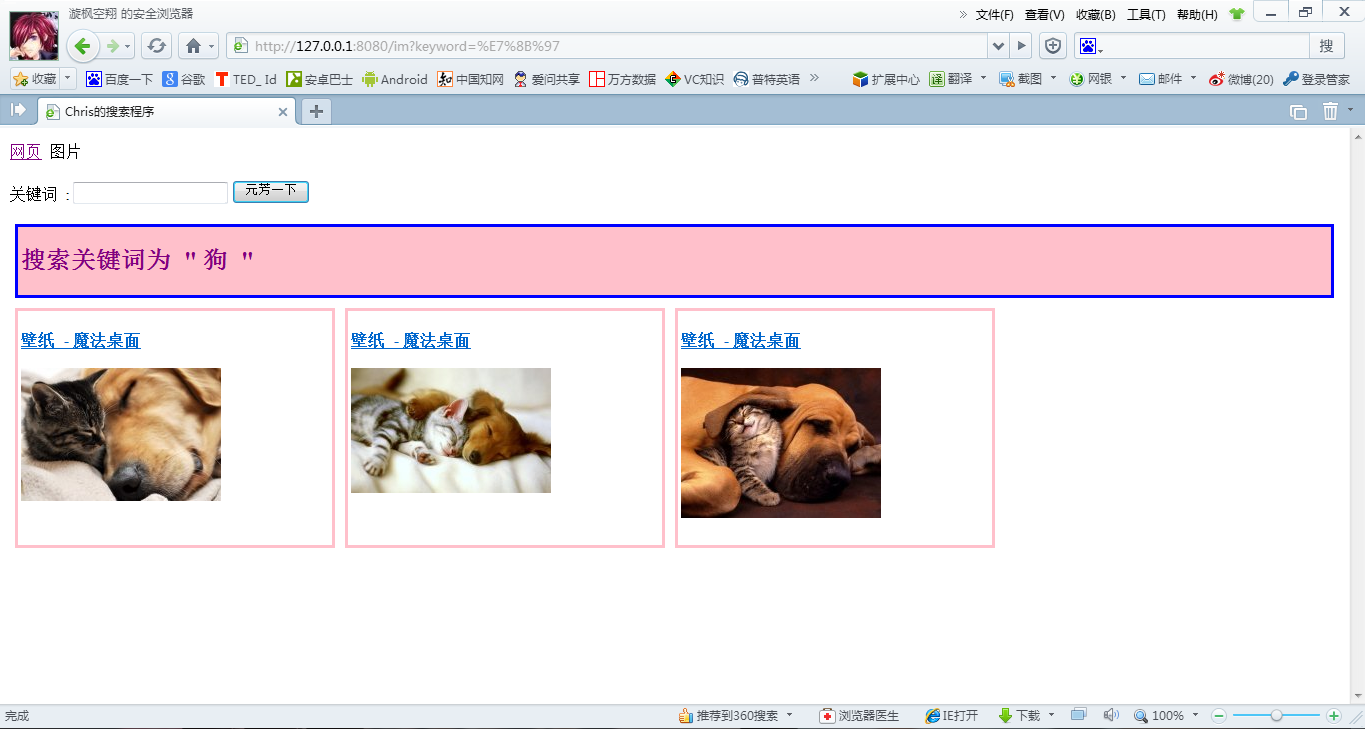
\includegraphics[width=10cm]{8.png}
\caption{the outcome of exercise 2.1.1 on the page}
\end{figure}
\subsection{Exercise 2.1.2 and 2.1.3}
Since these two exercises can be shown only using a piece of code, so I will display them together. Below are the codes:\\
\begin{lstlisting}[language=python,numbers=left,frame=leftline]
def get_page(page):
    return g.get(page, [])

def get_all_links(content):
    return content

def union_dfs(a,b):
    for e in b:
        if e not in a:
            a.append(e)

def union_bfs(a,b):
    for i in b:
        if i not in a:
            a.insert(0,i)

def crawl(seed, method):
    tocrawl = [seed]
    crawled = []
    graph = {}
    while tocrawl:
        page = tocrawl.pop()
        if page not in crawled:
            content = get_page(page)
            outlinks = get_all_links(content)
            graph[page]=outlinks
            globals()['union_%s' % method](tocrawl, outlinks)
            if method=='dfs':
                crawled.append(page)
            if method=='bfs':
                crawled.insert(0,page)
    if method=='bfs':
        crawled.reverse()
    return graph, crawled

g = {'A':['B', 'C', 'D'],\
     'B':['E', 'F'],\
     'D':['G', 'H'],\
     'E':['I', 'J'],\
     'G':['K', 'L']}

graph_dfs, crawled_dfs = crawl('A', 'dfs')
\end{lstlisting}
This experiment is quite easy, we only need to use some basic codes to achieve the function of print the graph in "bfs" method. Since it's easy to understand, I won't say much here. And these are the screen shots:\\
\begin{figure}[htbp]
\centering

\includegraphics[width=10cm]{2.png}
\caption{the outcome of exercise 2.1.2}
\end{figure}
\begin{figure}[htbp]
\centering
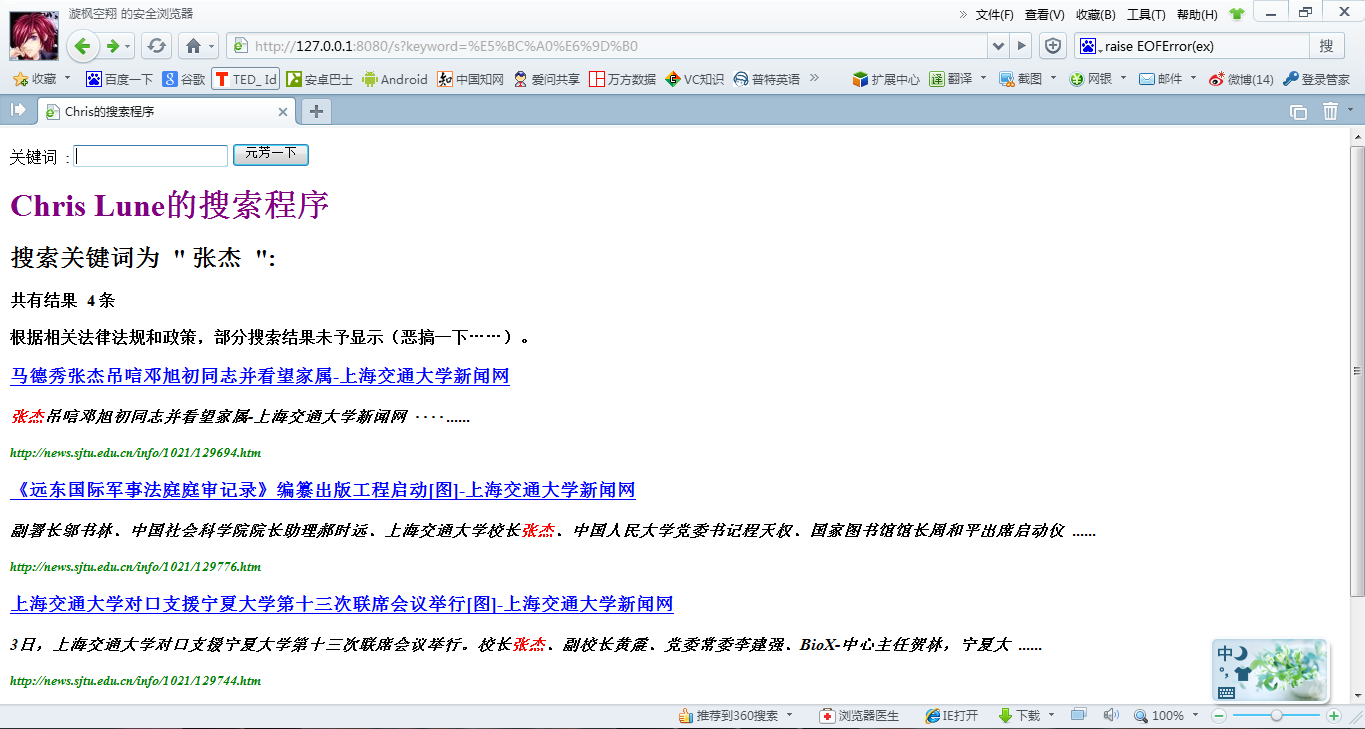
\includegraphics[width=10cm]{3.png}
\caption{the outcome of exercise 2.1.3}
\end{figure}
\subsection{Exercise 2.1.4}
This is the last part of the first half of experiment 2. At first , I thought it would be very difficult, but with the base of exercise 2.1.2 and exercise 2.1.3, it also becomes easy.\\
\begin{lstlisting}[language=python,numbers=left,frame=leftline]
from BeautifulSoup import BeautifulSoup
import urllib2
import re
import urlparse
import os
import urllib

def valid_filename(s):
    import string
    valid_chars = "-_.() %s%s" % (string.ascii_letters, string.digits)
    s = ''.join(c for c in s if c in valid_chars)
    return s

def get_page(page):
    content = ''
    import urllib2
    import socket
    try:
        content=urllib2.urlopen(page,timeout=10).read()
        return content
    except:
        print 'There is an error.'
        return 0

def get_all_links(content, page):
    import re
    import urlparse
    from BeautifulSoup import BeautifulSoup
    links = []
    tempset=set()
    soup=BeautifulSoup(content)
    for i in soup.findAll('a',{'href':re.compile(('^http|^/'))}):
        tempset.add(i['href'])
    for i in tempset:
        links.append(urlparse.urljoin(page,i))
    return links

def union_dfs(a,b):
    for e in b:
        if e not in a:
            a.append(e)

def union_bfs(a,b):
    for i in b:
        if i not in a:
            a.insert(0,i)

def add_page_to_folder(page, content):
    index_filename = 'index.txt'
    folder = 'html'
    filename = valid_filename(page)
    index = open(index_filename, 'a')
    index.write(page.encode('ascii', 'ignore') + '\t' + filename + '\n')
    index.close()
    if not os.path.exists(folder):
        os.mkdir(folder)
    f = open(os.path.join(folder, filename), 'w')
    f.write(content)
    f.close()

def crawl(seed, method, max_page):
    tocrawl = [seed]
    crawled = []
    graph = {}
    count = 0

    while tocrawl:
        page = tocrawl.pop()
        if page not in crawled and count<max_page:
            count+=1
            print page
            content = get_page(page)
            if content:
                add_page_to_folder(page, content)
                outlinks = get_all_links(content, page)
                globals()['union_%s' % method](tocrawl, outlinks)
                if method=='dfs':
                    crawled.append(page)
                if method=='bfs':
                    crawled.insert(0,page)
    if method=='bfs':
        crawled.reverse()
    return graph, crawled
\end{lstlisting}
In this part, what we need to do is to give out a certain number of links(url) by dfs or bfs. And we also need to handle some conditions where our request from crawlers are turned down by some websites. This is easy if we use "try...except...". And you can see the outcomes in the picture.\\
\begin{figure}[htbp]
\centering
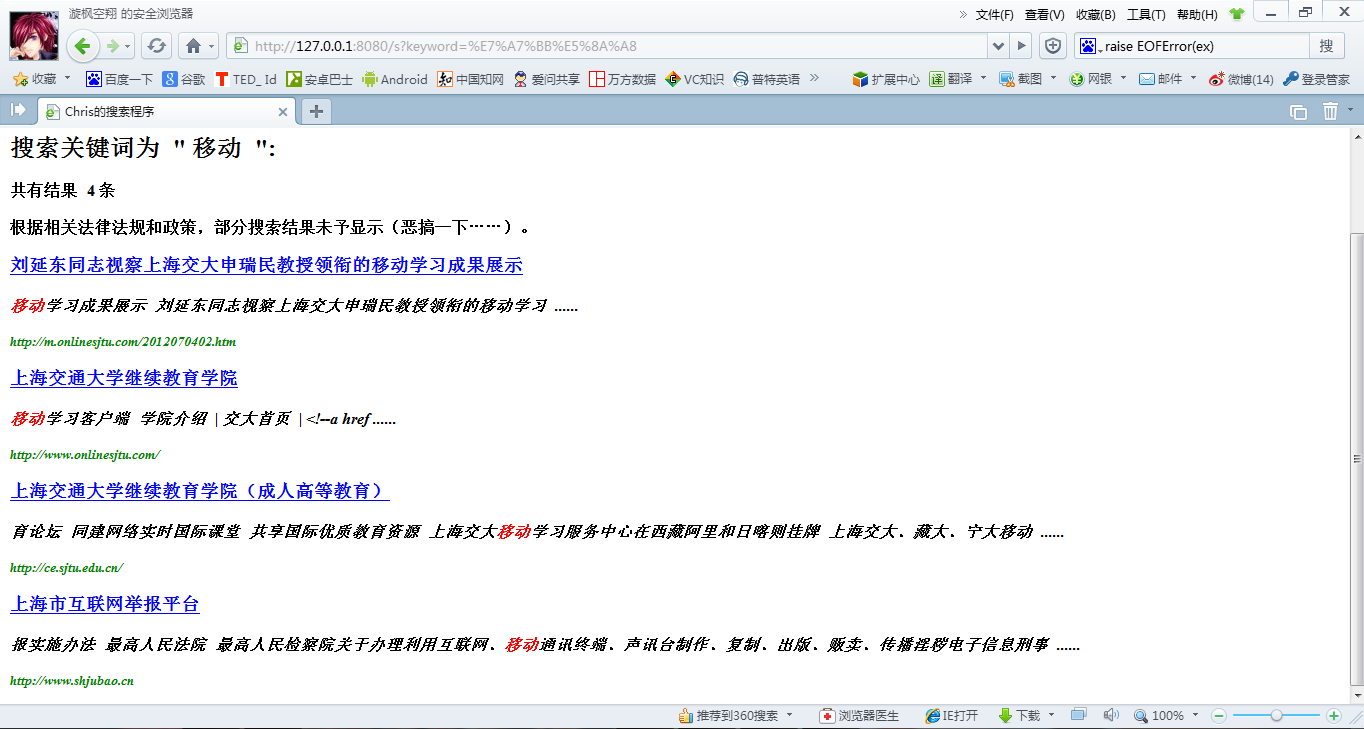
\includegraphics[width=10cm]{4.png}
\caption{the outcome of exercise 2.1.4}
\end{figure}
\subsection{Exercise 2.2.1}
I think this is hard for me to do. In my opinion, if we want to check the false positive rate of a BloomFilter, we can do it this way:
First, we check the number of all the different words in an article,e.g., we got A. Then we use an English dictionary to how many words in the dictionary are in the hashtable,e.g., we got B. Then (B-A)/B is the false positive rate.\\
But the fact shows that it is really hard. Not only can't we find such a big dictionary, but we also can't find some peculiar words such as names, writer-created words,etc. So though I get a dictionary with 370,000 words, it is still pretty funny that B is smaller than A.\\
So I just think of another way. I can find the rate by changing the capacity of the hashtable. For example, when the capacity of the hashtable is 100,000, then we got A as the number of different words shown in the article. Then we enlarge the hashtable to 1,000,000, and then we got number B. Then I think (B-A)/B can also represent the false positive rate of a BloomFilter.\\
And I will give out the code using the first method (I think it is the perfect method), while giving out the outcome of using my BloomFilter to try the article given in the experiment (named "pg1661.txt") in the second method( because I can only get it this way...)\\
And what I want to say is that we need to put the "pg1661.txt" and "dic.txt" in the root directory of disk D.\\
Here are the codes of the first method.\\
\begin{lstlisting}[language=python,numbers=left,frame=leftline]
import string
import re
class Bitarray:
    def __init__(self, size):
        """ Create a bit array of a specific size """
        self.size = size
        self.bitarray = bytearray(size/8)

    def set(self, n):
        """ Sets the nth element of the bitarray """

        index = n / 8
        position = n % 8
        self.bitarray[index] = self.bitarray[index] | 1 << (7 - position)

    def get(self, n):
        """ Gets the nth element of the bitarray """

        index = n / 8
        position = n % 8
        return (self.bitarray[index] & (1 << (7 - position))) > 0

    def find_in_hash(self,words):
        for i in range(5):
            num=BKDRHash(words,i)%1000000
            if self.get(num)!=1:
                return False
        return True

def BKDRHash(key,times):
    if times==0: seed=19
    if times==1: seed=171
    if times==2: seed=4513
    if times==3: seed=27137
    if times==4: seed=137519
    hash = 0
    for i in range(len(key)):
        hash = (hash * seed) + ord(key[i])
    return hash


if __name__ == "__main__":
    bitarray_obj = Bitarray(8000000)
    total_word=0
    f = open("D://pg1661.txt",'r')
    for line in f.xreadlines():
        for word in line.strip().replace("--"," ").split(' '):
            word=string.lower(word).replace(".","").replace(",","")
            if bitarray_obj.find_in_hash(word)!=True:
                total_word+=1
                for j in range(5):
                    num=BKDRHash(word,j)%1000000
                    bitarray_obj.set(num)
    dic_word=0
    dic=open("D://dic.txt",'r')
    for line in dic.xreadlines():
        for word in line.strip().split(' '):
            if bitarray_obj.find_in_hash(word):
                dic_word+=1
    dic.close()
    f.close()
    print total_word
    print dic_word
\end{lstlisting}
And I also got a failed screen shot of method 1, as you can see the words searched from the dictionary is smaller than the words found in the article. And the second graph is the outcome when I shrink the scale of the hash table to 100,000.\\
\begin{figure}[htbp]
\centering
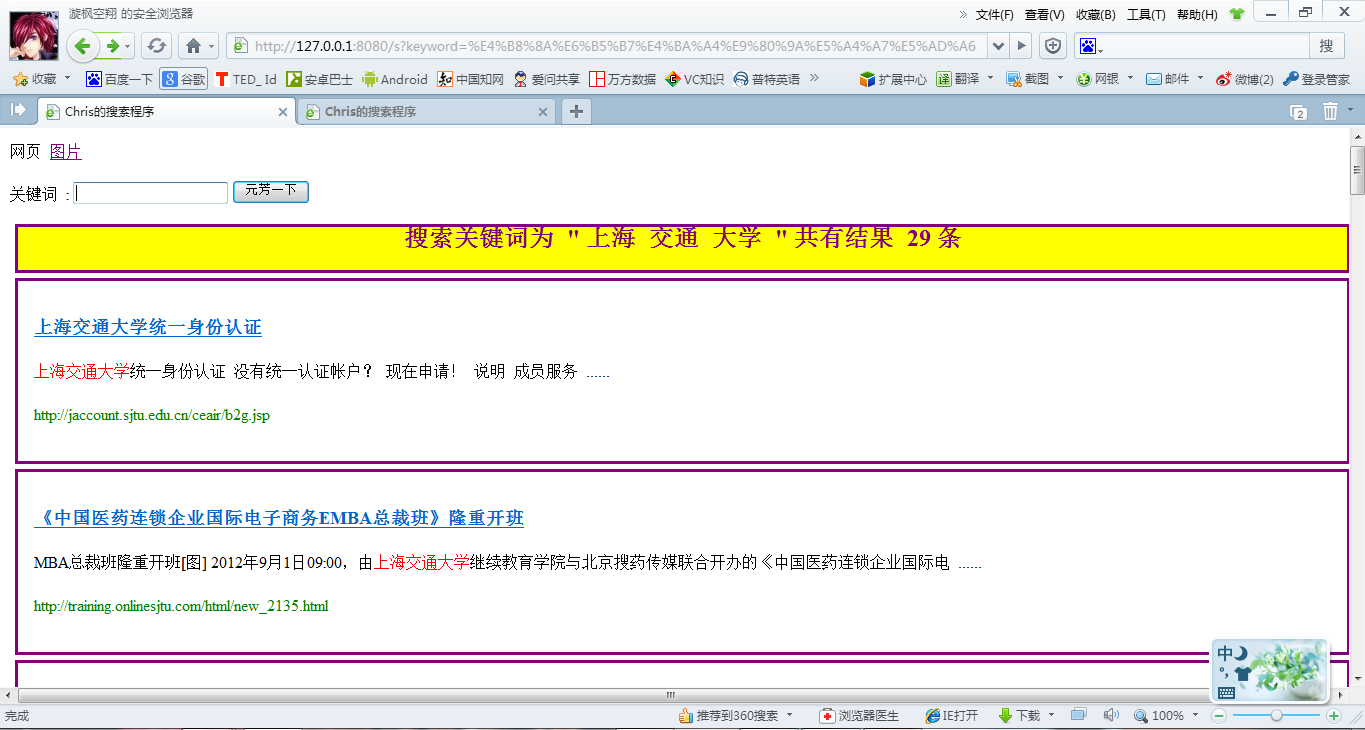
\includegraphics[width=10cm]{6.png}
\caption{the failed outcome of exercise 2.2.1 in method 1}
\end{figure}
\begin{figure}[htbp]
\centering
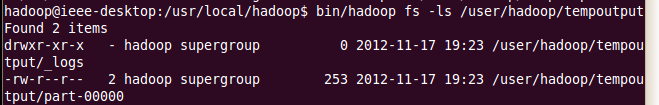
\includegraphics[width=10cm]{7.png}
\caption{the outcome of exercise 2.2.1 in method 2}
\end{figure}
And with the outcome I got , I estimate that the false positive rate of my BloomFilter is roughly 0.48%.\\
\subsection{Exercise 2.2.2}
Well, I have to admit that this is exactly the most difficult part in this experiment, since I have no concept of parrel crawler at all. And it's also hard for me to make out how the locks work and how to control the number of urls found by the crawler. Luckily, with a great effort, I narrowly understand a little of the working principle of threading. And below are my codes, the number of the thread can be changed by modify the variable "NUM" in the program.\\
I thought the example of the program is wrong at first, since whatever I do, I can't stop the processing when I get the exact number of the pages I want. Then once a while, I changed the last sentence to 't.join()', which means the thread is waiting for others to stop, and then it really stopped in the end. But I soon found that maybe it wasn't a good choice, since the teacher might want us to let the main thread wait others, not a subthread. So after so many times of trying to stop it, I found that it was because I didn't let all elements in the queue to get the 'taskdone' method that I couldn't kill the main thread. So after added some 'q.taskdone()' to my program, I sorted the problem easily.\\
\begin{lstlisting}[language=python,numbers=left,frame=leftline]
from BeautifulSoup import BeautifulSoup
import urllib2
import re
import urlparse
import os
import urllib
import socket
import threading
import Queue
import time


def valid_filename(s):
    import string
    valid_chars = "-_.() %s%s" % (string.ascii_letters, string.digits)
    s = ''.join(c for c in s if c in valid_chars)
    return s

def get_page(page):
    time.sleep(0.5)
    try:
        content=urllib2.urlopen(page,timeout=10).read()
        return content
    except:
        #There is an error.#
        return []

def get_all_links(content, page):
    if content==[]:
        return []
    links = []
    tempset=set()
    soup=BeautifulSoup(content)
    for i in soup.findAll('a',{'href':re.compile(('^http|^/'))}):
        tempset.add(i['href'])
    for i in tempset:
        links.append(urlparse.urljoin(page,i))
    return links

def add_page_to_folder(page, content):
    index_filename = 'index.txt'
    folder = 'html'
    filename = valid_filename(page)
    index = open(index_filename, 'a')
    index.write(page.encode('ascii', 'ignore') + '\t' + filename + '\n')
    index.close()
    if not os.path.exists(folder):
        os.mkdir(folder)
    f = open(os.path.join(folder, filename), 'w')
    f.write(content)
    f.close()

def working():
    page_num=0
    while page_num<10:
        page = q.get()
        if page not in crawled:
            content = get_page(page)
            outlinks = get_all_links(content,page)
            if outlinks==[]:
                q.task_done()
                continue
            print page
            page_num+=1
            for link in outlinks:
                q.put(link)
            if varLock.acquire():
                crawled.append(page)
                varLock.release()
                q.task_done()
            else:
                q.task_done()
        else:
            q.task_done()
    while q.empty()==False:
        q.get()
        q.task_done()

NUM = 3
crawled = []
graph = {}
varLock = threading.Lock()
q = Queue.Queue()
q.put('http://www.sjtu.edu.cn')
for i in range(NUM):
    t=threading.Thread(target=working)
    t.setDaemon(True)
    t.start()
q.join()
print "That's all you want."
\end{lstlisting}
And I also set that each thread searches 10 urls, you can change it to the number you want in "while" circuit.\\
Here is the screen shot.\\
\begin{figure}[htbp]
\centering
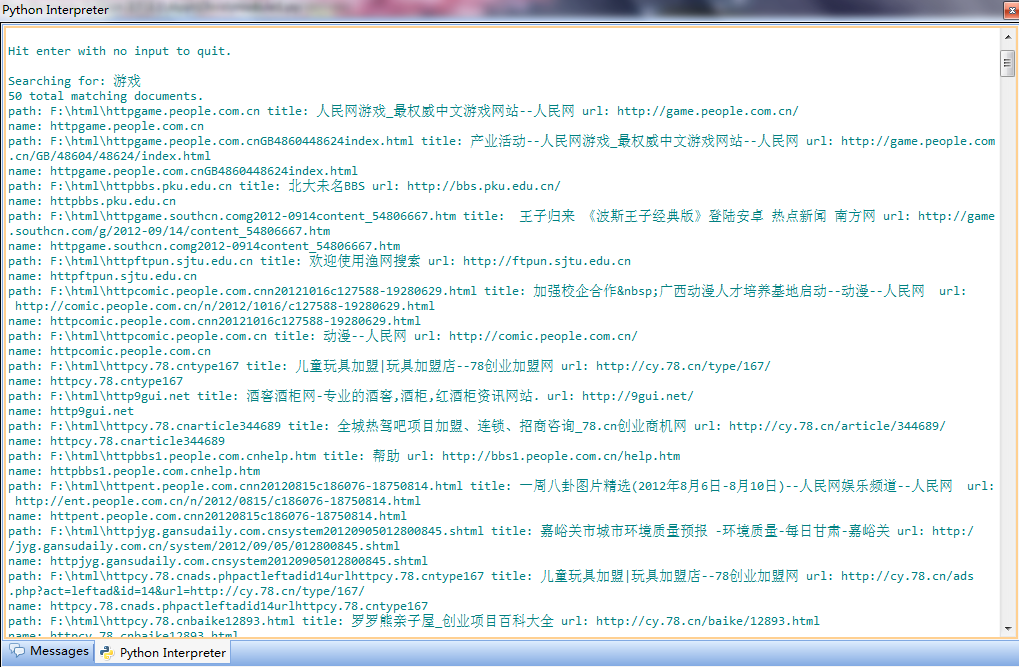
\includegraphics[width=10cm]{5.png}
\caption{the outcome of exercise 2.2.2}
\end{figure}
\section{The Problems I Met in the Experiment}
As I have said above, there are so many problems when I try to do the experience. The first is coding problem ,but I found that when I got the wrong code, I only need to change it to 'gbk' code. The second problem is to find a dictionary to get all different words in an article. However, I failed on it. But I will still try to solve the problem in the future. The third problem is the threading and lock problem. Luckily, I found a lot of introduction of them on the Internet, and then I finally make out how they works. \\
But I still have to say, it is a really hard thing to achieve the experiment...\\
\section{Some of My Thoughts}
I like the first experiment of the first half very much. Because it gives us a chance to give out or modify some information just using python, without a browser. And I'd like to try to give out my micro-blogs using this method. And I also think the second half of the experiment is a inspiration. With it, we can easily count and memorize different information in an article or on the website. And the multiple threading programming also make it faster for us to get the information or urls we need. Now I am just indulged in the magical programming using python. And though it is a hard thing, I really have fun.
\end{document}
